

{Up till now, all I have done is to try to understand the nature of the brachistiochrone problem and its solution. I have explored various parametric equations that describe the curve of fastest descent, but I now would like to apply it to a real problem with real coordinates to define a real curve from real points to further investigate the curve and the time taken for a spherical mass to slide this curve-path.}

{I would now explore the brachistochrone curve for the points $A(x_{1},y_{1})$ and $B(x_{2},y_{2})$, where $x_{1} = 0, y_{1} = 0, x_{2} = 4$ and $y_{2} = -3$. Before evaluating the problem, we would like that the beginning point of the curve be placed at the peaks of the cycloid as this ensures that the mass sliding through the curve would attain the highest velocity (as the tangent at the initial point would be a vertical line), However this requires that the parametric equations to be of $\theta\in2\pi n$, where $n\in\mathbb{Z}^{+}$.}

{Therefore by inputting the values of $x_{2}$ and $y_{2}$ we have,}

	\begin{equation}
		4 = r\left(\theta - \sin\theta\right)
		\label{x2eq}
	\end{equation}

	\begin{equation}
		-3 = r\left(1 - \cos\theta\right)
		\label{y2eq}
	\end{equation}

{Implies,}

	$$r = \frac{4}{\theta - \sin\theta}$$

{Substituting the value for \textit{r} in \ref{y2eq}, we have,}

	$$-3 = \left(\frac{4}{\theta - \sin\theta}\right)\left(1 - \cos\theta\right)$$

{Implies,}

	$$3\left(\sin\theta - \theta\right) = 4\left(1 - \cos\theta\right)$$

{Solving for $\theta$ using a GDC, we have, $\theta = -2.87995$. Therefore we have,}

	$$r = \frac{4}{-2.87995 - \sin -2.87995} \approx -1.52597$$

{Sustituting this value of \textit{r} in equations \ref{cyceq}, we have,}

	$$x = -1.53\left(\theta - \sin\theta\right)$$

	$$y = 1.53\left(1 - \cos\theta\right)$$

{Plotting the above parametric equations on Desmos we get,}

\begin{figure}[H]
\centering
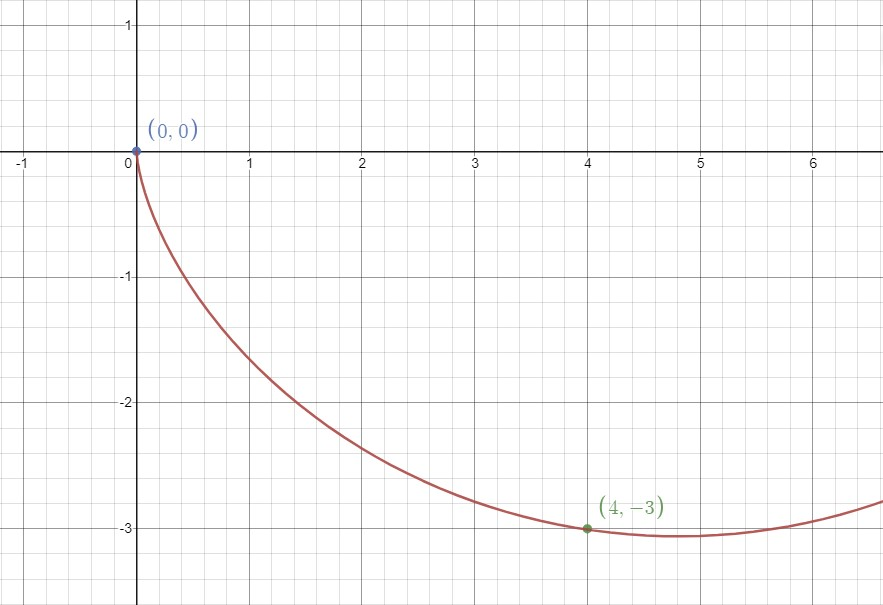
\includegraphics[width=15cm]{cycplt.jpg}
    		\caption{{Plot of the parametric equations that plot the cycloid}}
\end{figure}

{As we can see, the above curve passes through the points $A(0,0)$ and $B(3,-4)$}

{Using equation \ref{Tcal}, we can find the time taken for an object/mass to slide from the initial point, to the final point, ie. the the points $A(0,0)$ and $B(3,-4)$. Therefore the time it takes to reach from the initial to the final point is,}

{If I am to consider each point to be in the units of meters, then we have,}

	$$T = \left|\sqrt{\frac{-1.52597}{-9.81}}\cdot -2.87995\right|$$

{Therefore,}

	$$T \approx 1.13586 s$$

{This time is relatively much shorter than if an object were to slide down a ramp from point $A(0,0)$ to $B(3,-4)$.}

% Valididty through Simulation 

{What I had done above could be classified as simple mathematical substitution, therefore to explore the validity of my answers, I had used a simulation scripted in Python (“The Brachistochrone Problem”) to numerically integrate using an algorithm known as the Runge-Kutta Fourth Order, simply RK4 to find and estimate what is the shortest time taken for an object to slide through a curve and then finally compare those results with our estimated results found above, in an attempt to prove the credibility of our results.}

{From the simulation, that I used to numerically integrate and estimate the values of the time it takes for various curves. I had created a graph with the time it takes for specific curves for our specific case.}

\begin{figure}[H]
\centering
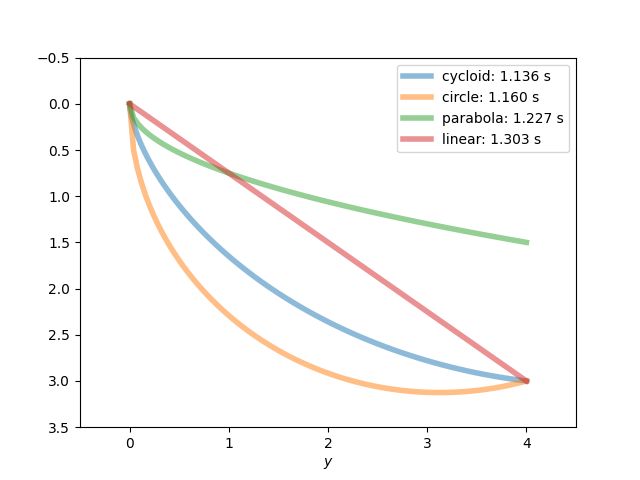
\includegraphics[width=15cm]{BrachDia.png}
    		\caption{{Plot from the simulation graphically showing various curves and the time it takes for descent}}
\end{figure}

{From the above graph, it is clear that, the cycloid is the curve of fastest descent as it takes the cycloid approximately 1.136 seconds where as it takes 1.303 seconds for a linear curve. This result is also consistent with my findings, as both the simulation results and the mathematically derived results through equations are the same.}


